%\documentclass[12p]{article}
%\usepackage{a4paper,makeidx}
%\usepackage[dvips]{graphics}
\documentclass{article}
\usepackage{graphicx}
\usepackage{subfig}
\usepackage{multirow}

%\documentclass[smallextended]{svjour3}
%\usepackage[dvips]{graphicx}
%\usepackage{subfig}
%%%%%%%%%%%%%%%%%%%%%%%%%%%%%%%%%%%%%%%%%%%%%%%%%%%%%%%%%%%%%%%%%%%%%%%%%%%%%%%%%%%%%%%%%%%%%%%%%%%%%%%%%%%%%%%%%%%%%%%%%%%%

\righthyphenmin=55
\newlength{\gnat}
\newlength{\figheight}
\newlength{\figwidth}
\setlength{\textwidth}{6in}
\setlength{\evensidemargin}{0.2in}
\setlength{\oddsidemargin}{0.2in}
\setlength{\topmargin}{0.0in}
\setlength{\textheight}{9in}
\setlength{\headsep}{10pt}
\setlength{\columnsep}{0.375in}

\newtheorem{theorem}{Theorem}
\newtheorem{proposition}{Proposition}
\newtheorem{lemma}{Lemma}
\newtheorem{corollary}{Corollary}
\newtheorem{definition}{Definition}
\newtheorem{remark}{Remark}
\newtheorem{claim}{Claim}

\def\IR{\Bbb R}
\def\tF{{\tilde F}}
\def\tG{{\tilde G}}
\def\tE{{\tilde E}}
\def\hF{{\hat F}}
\def\hG{{\hat G}}
\def\hE{{\hat E}}
\def\oF{{\overline{F}}}
\def\oG{{\overline{G}}}
\def\CC{{\cal C}}
\def\uF{{\underline{F}}}
\def\uG{{\underline{G}}}
\def\oC{{\overline{C}}}
\def\uC{{\underline{C}}}
\baselineskip= 20pt
%\input{tcilatex}

\begin{document}

\title {Random time transformation analysis of Covid19 2020 \\
WORKING DRAFT. PLEASE DON'T DISTRIBUTE
}

\author {
Nitay Alon
\\
{\em E-mail: \tt{nitayalon@mail.tau.ac.il}} \\
Isaac Meilijson
\\
{\em E-mail: \tt{isaco@tauex.tau.ac.il}} \\
{\em School of Mathematical Sciences} \\
{\em Raymond and Beverly Sackler Faculty of Exact Sciences} \\
{\em Tel-Aviv University, 6997801 Tel-Aviv, Israel} \\
}

%\titlerunning{Covid19 2020}
%\authorrunning{Alon and Meilijson}

\maketitle

\pagenumbering{arabic}

\begin{abstract}
\noindent The SIR epidemiological equations model new affected and removed cases as roughly proportional to the current number of infected cases. The present report adopts an alternative that has been considered in the literature, in which the number of new affected cases is proportional to the $\alpha \le 1$ power of the number of infected cases. After arguing that $\alpha=1$ models exponential growth while $\alpha<1$ models polynomial growth, a simple method for parameter estimation in differential equations subject to noise, the random-time transformation RTT of Bassan, Meilijson, Marcus and Talpaz 1997, will be reviewed and applied in an attempt to settle the question as to the nature of Covid19.

%\keywords{
%\noindent{\bf JEL Classification Numbers:}
%
\end{abstract}

%\vspace{1cm}

%\noindent \hrulefill \hspace{12cm}

%\baselineskip= 20pt

%\newpage

\section{Introduction} \label{introduction}

\noindent {\bf The SIR epidemiological model}. Let $S(t) = K - X(t)$ be the number of susceptible cases at time $t$, expressed in terms of the number of affected cases $X(t)$ and the possibly unknown parameter $K$ (that may or may not be the population size $N$ usually substituted for $K$). Let $R(t)$ be the removed cases at time $t$, dead
% ($V(t)$)
or recovered.
%($W(t)=R(t)-V(t)$).
Let $I(t)=S(t)-R(t)$ be the number of infected cases at time $t$. The common formulation of the SIR (Susceptible, Infected, Removed) epidemiological model is the variant of the system of ODE
\begin{eqnarray}
dX(t) & = & \beta(t) g(I(t)) \max(0,1 - X(t)/K) dt \label{DEforX} \\
dR(t) & = & \gamma I(t) dt \label{DEforR} \\
I(t) & = & \max(0,X(t)-R(t)) \label{eqforI}
\end{eqnarray}
where $K=N$ and $g(x)=x$. The parameter $\beta(t)$ is generally estimated by smooth local regression of \linebreak $X$-increments with respect to the RHS of (\ref{DEforX}). The basic reproduction number $R_0={{\beta(t)} \over \gamma}$ is of primary importance, as its transition from above to below $1$ indicates whether the epidemic is spreading or dwindling, whether the number of infected cases $I$ increases or decreases with time.

\bigskip

%At the early stages of the epidemic, the substitution of $K$ by population size $N$ or anything big enough including $\infty$, has similar effects, modelling essentially exponential growth if $g(x)=x$.
Equations (\ref{DEforR}) and (\ref{eqforI}) as well as the linear appearance of the susceptible cases in (\ref{DEforX}) are quite straightforward under a stationary regime, but the role of $I(t)$ in (\ref{DEforX}) needs some attention. The effective vicinity of a susceptible case need not be the entire infected cohort, just as the asymptote of affected cases need not be population size $N$.

This report will illustrate on the Covid19 2020 data that
%if $K$ is allowed to be a free parameter,
the SIR system of equations may accept an almost exact solution in which $\beta$ (and not only $\gamma$) is constant, provided $g(\cdot)$ is modelled as $g(x)=x^\alpha$
for some $\alpha<1$ as has been repeatedly suggested in the literature (see Bj{\o}rnstad, Finkenst\"{a}dt and Grenfell in their various publications, such as \cite{AAA} and the references therein).

$K$ is the asymptote to which the number $X$ of affected cases converges, the maximal sub-population size to become affected. This scenario-dependent random object $K$ will be treated as a parameter.

Had the function $g$, modelling the impact of the current extent of infection on the emergence of new cases, been known, parameter estimation via these differential equations would have provided (unjustifiably) accurate estimates of the asymptote $K$. Once $g(x)=x$ is rejected in favor of \linebreak $g(x)=x^\alpha$ for some $\alpha<1$, this shape parameter $\alpha$ has to be estimated together with $(K , \beta, \gamma)$, and the overall effect on $K$ is less clear-cut.

%The Covid19 2020 indicates country by country that the data from March to May 2020 induced rather stationary behavior, with $K$ values generally strongly significantly finite, not exceeding three times the number of affected cases at the end of May 2020, with $\alpha$ values roughly between $0.5$ and $0.7$, with $\alpha=1$ off limits. The model $g(x)=x$ is adopted throughout.

\bigskip

\noindent {\bf Exponential or asymptotically constant growth?} The cases $\alpha=1$ and $\alpha<1$ are not just variations on a mathematical abstraction. This dichotomy differentiates in principle between exponential and sub-exponential growth. If population is infinite,

The $\alpha=1$ equations
\begin{eqnarray}
d X(t) & = & \beta (X(t)-R(t)) dt \label{DEforX1} \\
d R(t) & = & \gamma (X(t)-R(t)) dt \label{DEforR1}
\end{eqnarray}
i.e., $d I(t) = (\beta-\gamma) I(t) dt$, lead to $I(t)=I(0)\exp\{(\beta-\gamma)t\}$, and then $X(t)=X(0)\exp\{\beta t\} \ , \ \linebreak R(t)=R(0)\exp\{\gamma t\}$. This is exponential growth.

The $\alpha<1$ equations
\begin{eqnarray}
dX(t) & = & \beta (X(t)-R(t)^\alpha dt \label{DEforX1} \\
dR(t) & = & \gamma (X(t)-R(t)) dt \label{DEforR1}
\end{eqnarray}
i.e.,
\begin{equation} \label{DEforI}
d I(t) = (\beta I(t)^\alpha - \gamma I(t))dt
\end{equation}
admit a constant solution
\begin{equation} \label{Isub0}
I(t) \equiv I_0 = ({\beta \over \gamma})^{1 \over {1-\alpha}}
\end{equation}
under which
\begin{equation} \label{slopes}
X(t) \approx X(0)+{{\beta^{1 \over {1-\alpha}}} \over {\gamma^{\alpha \over {1-\alpha}}}} t  \ ; \ R(t) \approx R(0)+{{\beta^{1 \over {1-\alpha}}} \over {\gamma^{\alpha \over {1-\alpha}}}} t
\end{equation}
are parallel linear functions. I.e., new affected cases and new removed cases are invariant in time, with an invariant level of infected cases.
This is asymptotically linear growth of the cumulative number of affected cases, with an initial convex polynomial behavior.

\bigskip

But population size is finite, and the target sub-population may be even smaller. If Equation (\ref{DEforX1}) is replaced by Equation (\ref{DEforX}) with $K$ re-incorporated and $g(x)=x^\alpha$, solutions invariably show the typical Covid19 behavior of empirical data, number of infected cases $I(t)$ that rather than converge to $I_0$ defined in (\ref{Isub0}), increase to a maximum (for which $I_0$ is a sort of upper bound) and then decrease, towards zero hopefully.

A word of warning explaining "a sort of", all parameters are estimated jointly under the given empirical data. It is not clear that these parameters, especially $\beta$, apply verbatim to other \linebreak $K$-scenarios. Take into account also that there are other built-in assumptions throughout, that recovered cases become immune, and prevailing conditions don't change. These are issues for further thought.

All countries analyzed in the sequel based on data until early June 2020, with the possible exception of those with insufficient data, display $\alpha$ values far below $1$ (and $K$ values far below $N$). The profile likelihood function of $\alpha$ is generally quite flat, so $\alpha$ is somewhat noisily estimated.

At the end of May 2020 most countries and the world as a whole displayed number of infected cases increasing with time, making estimation more speculative than for countries where the basic reproduction number $R_0$ crossed already below $1$.

\bigskip

Figure \ref{log075}, based roughly on Brazil data analysis, displays the logarithm of the theoretical solution to the SIR equations for $500$ days with $\alpha=0.75$, $\beta=2$, $\gamma=0.05$ and arbitrarily chosen $K=500.000$. Figure \ref{log1} preserves $K$ and $\gamma$ from Figure \ref{log075} as well as the initial condition of one affected case, but sets $\alpha=1$. The value of $\beta$ was calibrated as $0.125$ so that the maximal number of infected cases will mimic that of Figure \ref{log075}.

Figures \ref{france}, \ref{germany} and \ref{italy} display the logarithms of the empirical number of affected and infected cases in France, Germany and Italy respectively. The observed data conform with the sub-exponential growth represented by $\alpha<1$.

\begin{figure}
\begin{center}
%\subfloat [Second-chance model and absolute standard normal]
{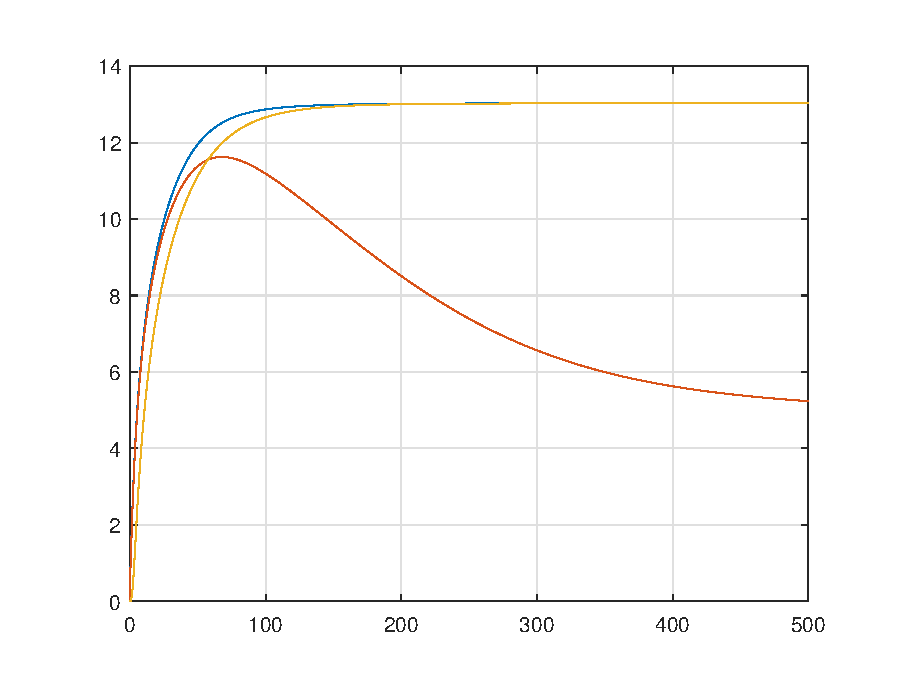
\includegraphics[width=4in,height=2in]{log075.eps}}
% \qquad
%{\includegraphics[width=2in,height=2in]{Fig3.eps}}
\end{center}
%\begin{center}
\caption{Logarithm of affected, infected and removed cases under $\alpha=0.75 \ , \ \beta=2 \ , \ \gamma=0.05$  and $K=500.000$}
%\end{center}
\label{log075}
\end{figure}

\begin{figure}
\begin{center}
%\subfloat [Second-chance model and absolute standard normal]
{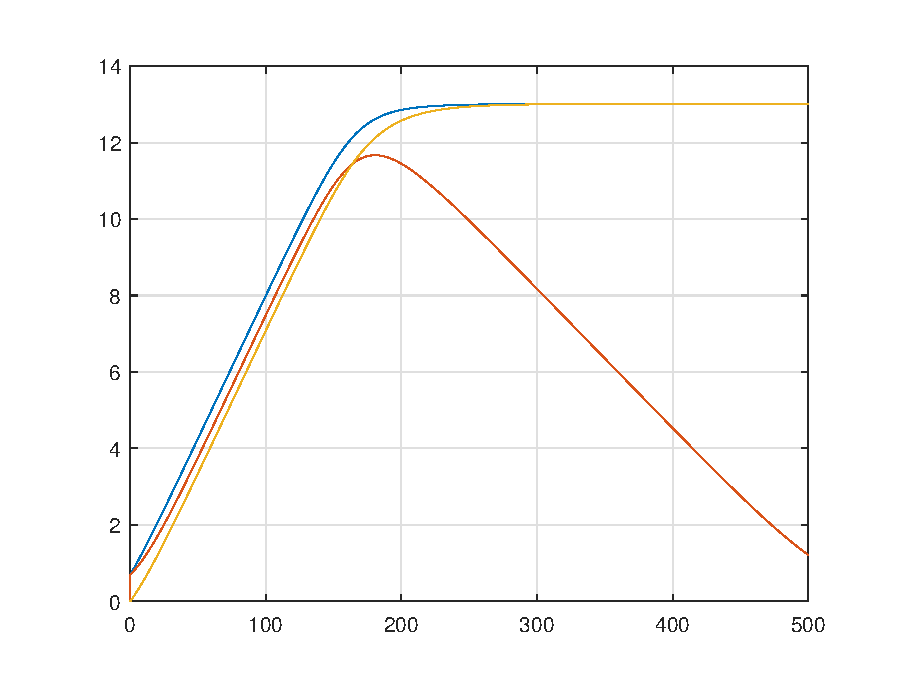
\includegraphics[width=4in,height=2in]{log1.eps}}
% \qquad
%{\includegraphics[width=2in,height=2in]{Fig3.eps}}
\end{center}
%\begin{center}
\caption{Logarithm of affected, infected and removed cases under $\alpha=1 \ , \ \beta=0.125$, $\gamma=0.05$ and $K=500.000$}
%\end{center}
\label{log1}
\end{figure}

\bigskip

\begin{figure}
\begin{center}
%\subfloat [Second-chance model and absolute standard normal]
{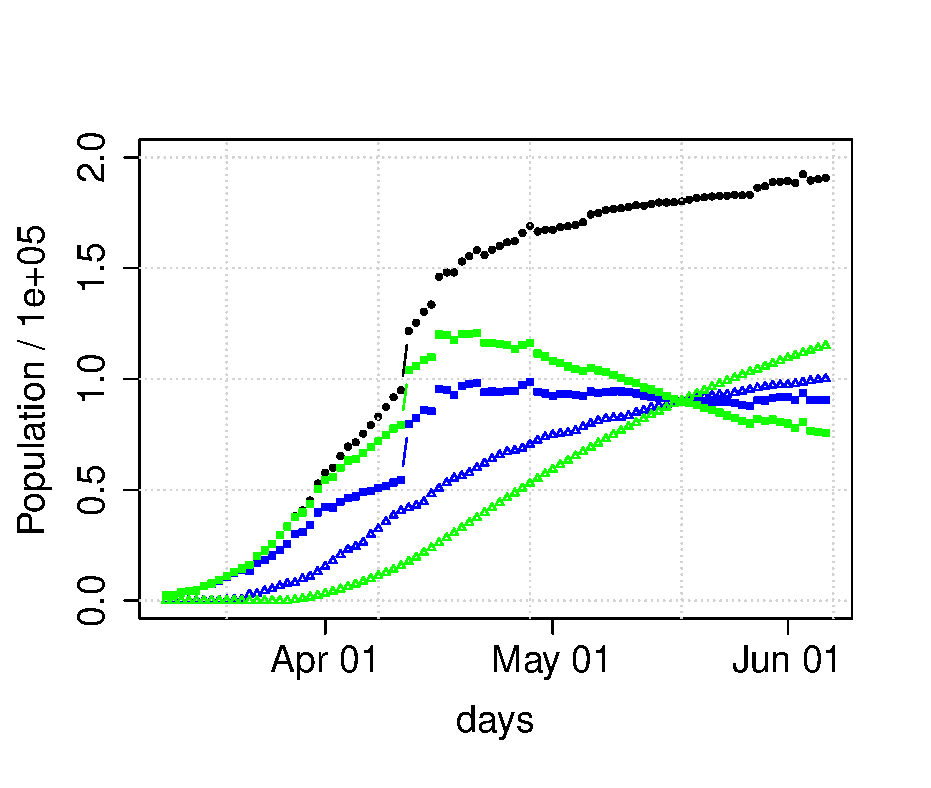
\includegraphics[width=4in,height=2in]{france.eps}}
% \qquad
%{\includegraphics[width=2in,height=2in]{Fig3.eps}}
\end{center}
%\begin{center}
\caption{Logarithm of affected and infected cases in France, March to May 2020}
%\end{center}
\label{france}
\end{figure}

\begin{figure}
\begin{center}
%\subfloat [Second-chance model and absolute standard normal]
{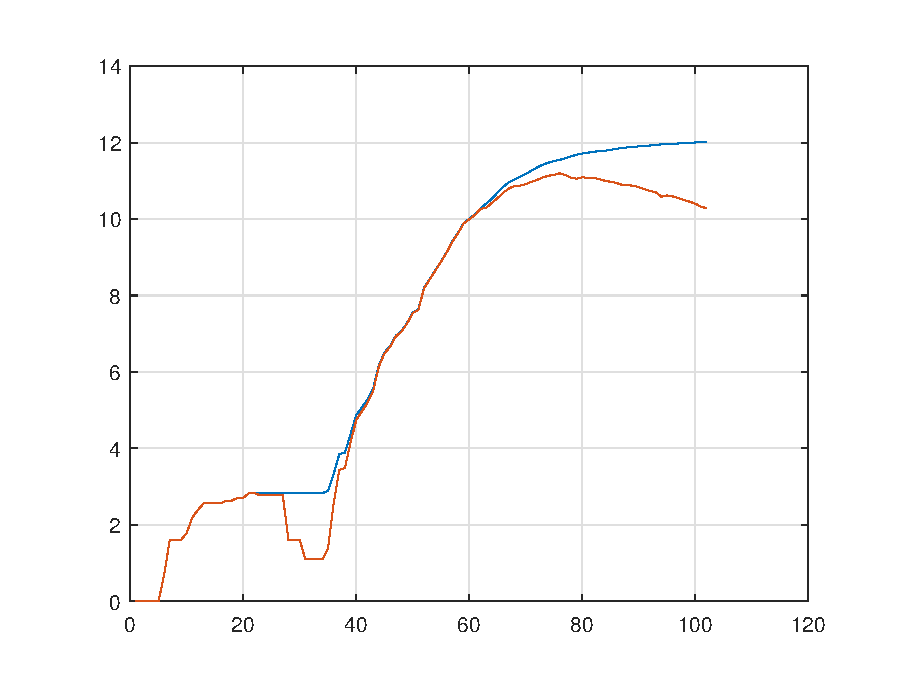
\includegraphics[width=4in,height=2in]{germany.eps}}
% \qquad
%{\includegraphics[width=2in,height=2in]{Fig3.eps}}
\end{center}
%\begin{center}
\caption{Logarithm of affected and infected cases in Germany, March to May 2020}
%\end{center}
\label{germany}
\end{figure}

\begin{figure}
\begin{center}
%\subfloat [Second-chance model and absolute standard normal]
{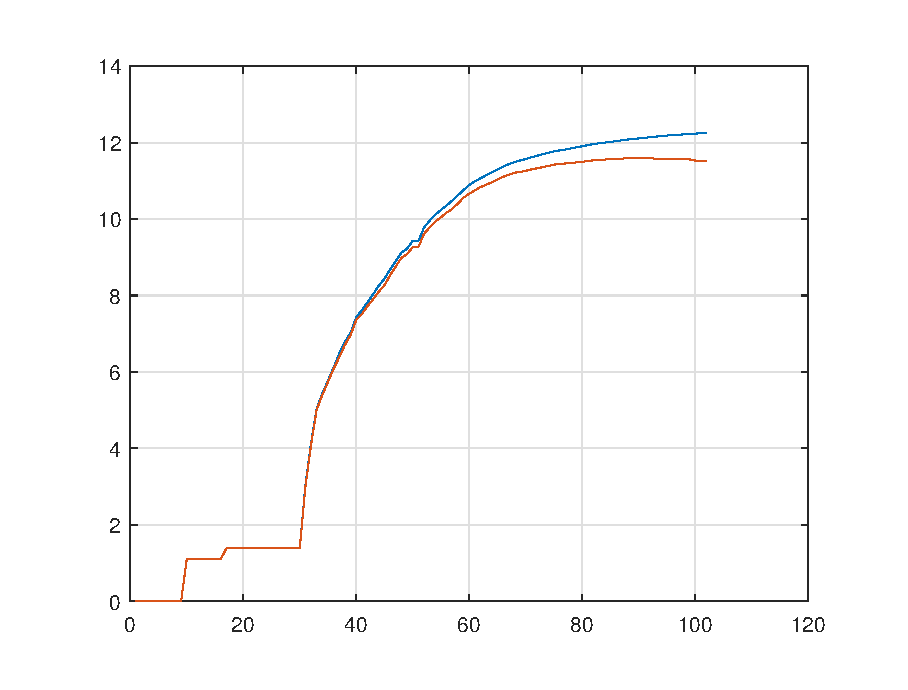
\includegraphics[width=4in,height=2in]{italy.eps}}
% \qquad
%{\includegraphics[width=2in,height=2in]{Fig3.eps}}
\end{center}
%\begin{center}
\caption{Logarithm of affected and infected cases in Italy, March to May 2020}
%\end{center}
\label{italy}
\end{figure}

\noindent {\bf Remark on the $R_0$ transition below $1$}. It is quite popular these days to welcome this transition, wrongly referred to as leaving behind exponential growth in favor of a period of recovery. This transition occurs at the moment when the number of infected cases is at a maximum, where care should be perhaps strengthened rather than relaxed. All graphs above show that the recovery period until the number of infected cases is at a safer low level "in the current wave", is long and slow.  The USA is at the transition point in early June, but if conditions stay stationary, the current wave is predicted to be still at unsafe levels in October. Germany and Italy will experience unsafe levels at least until the end of August.

\section{Preliminary data handling and analysis} \label{preliminarysection}

Equation (\ref{DEforR}) expresses the reasonable premise that new removed cases are proportional to the number of infected cases. I.e., the cumulative number $R$ of removed cases should be proportional to the cumulative sum of currently infected cases. A linear regression with slope $\gamma$ and zero intercept should manifest this relationship. After checking that this is roughly so, the empirically measured affected cases $X$ are kept intact but its division into removed cases $R$ and infected cases $I$ is modified minimally so that the regression relation will hold. The method by which this has been done can be found in the Appendix. Figures NNN display the raw and modified data for a number of countries. This regression provides an initial estimate for $\gamma$, illustrated in Table \ref{tabl}.

\bigskip

Equation (\ref{DEforI}) states that early in the epidemic $dI(t) \approx \beta (I(t))^\alpha$ or ${{(I(t))^{1-\alpha}} \over  {1-\alpha}} \approx \beta (t-t_0)$ for some $t_0$. Warned by the noisy early behavior evident in Figures \ref{france}, \ref{germany} and \ref{italy}, let Day$1$ be the date when the number of infected cases first reaches, say, $400$ cases, and let Day$2$ be the date when the number of infected cases first reaches, say, one third of the maximal observed number of infected cases. The parameter $\alpha$ can be initially estimated from this data time range by the value that maximizes the correlation coefficient between $(I(t))^{1-\alpha}$ and time. If this correlation coefficient is close enough to $1$, the $\alpha$-model can be adopted, and the date $t_0$ when the epidemic started, can be assessed, together with $\alpha$ and $\beta$. Table \ref{tabl} illustrates some results of this preliminary analysis as $\alpha_1$ and $\beta_1$. Correlation coefficients are not reported, but all nine came out $0.99$ and above.

By equation (\ref{DEforX}), on this time interval from Day$1$ to Day$2$ the increments of $X$ should equal approximately $\beta I^\alpha$. In other words, the logarithm of (a centered week-long moving average of) the daily increments of $X$ should satisfy the linear regression $\log(\beta)+\alpha \log(I)$. The corresponding regression estimates of $\alpha$ and $\beta$ are illustrated in Table \ref{tabl} as $\alpha_2$ and $\beta_2$.

The purpose in performing this preliminary analysis is to display in simple terms that data does indeed conform to the SIR model augmented by the introduction of $\alpha$, avoiding still the issue of $K$. No attempt to attach significance statements to these findings is followed at this preliminary stage. That will be the role of the RTT likelihood model.

\begin{table}
\begin{center}
\begin{tabular}{l|cccccccc|r}
Country & $\alpha_1$ & $\beta_1$ & $\alpha_2$ & $\beta_2$ & $\gamma$ & Day$1$ & Day$2$ & Start  & \\ \hline
Belgium & 0.78  & 1.3469   & 0.70   & 2.9703  & 0.0035   &  36  & 62   & 24 &   \\
Brazil  & 0.59    &4.1448       &  0.72     & 2.1864   & 0.0540   & 58   & 104 & 52      &   \\
Chile   & 0.31 &16.940 &0.57 &  3.929 & 0.0450 & 59 & 106 & 54 &  \\
France  & 0.73 & 1.861 &  0.77& 1.544 &0.0278 & 44 & 67 & 34 & \\
Germany & 0.42 & 43.781&0.40 & 76.869 & 0.0621 & 51 & 62 & 50 &  \\
Israel & 0.75 &  1.820& 0.30 & 52.137 & 0.0379& 60 & 67 & 51 & \\
Italy  & 0.78 & 1.268& 0.77 & 1.666 & 0.0255 & 35 & 58 & 23 & \\
Sweden &0.77 &0.558 & 0.69 & 1.321 & 0.0181 & 50 & 77 & 19 &    \\
USA   & 0.85 &1.070 & 0.80 &1.936 &0.0116 & 46 & 74 & 32 &   \\ \hline
\end{tabular}
\caption{
Initial parameter estimates and time ranges
\label{tabl}
}
\end{center}
\end{table}


\bigskip

Data for the above and further analysis, taken from the COVID-19 Data Repository of
the Center for Systems Science and Engineering (CSSE) at Johns Hopkins
University, consist of the empirical $X$ data and the modified $I$ and $R$ data, from Day$1$ onwards.

The next section will introduce parameter estimation of $K,\alpha, \beta,\gamma$ under the SIR equations.

\section{RTT applied to Covid19 2020} \label{RTTsection}

The paradigm to be adopted is that $\alpha$ is a (possibly location-dependent) characteristic of the condition, while $K$ is a local-scenario parameter that reflects behavior and regulatory measures. It is important to estimate all parameters jointly in order to obtain as accurate an estimate of $\alpha, \beta, \gamma$ as feasible. This will allow the calculation of $I_0$ in (\ref{Isub0}) as an estimated upper bound (corresponding to an infinite population) on the ongoing number of infected cases as well as of the slope of the linear functions in (\ref{slopes}), the condition incidence per unit time.

%\bigskip

%The data for Italy and USA place $\alpha$ around $0.55$. For now, $\alpha$ will be estimated by MLE $\hat{\alpha}$ country by country. Perhaps the analysis will lead to a reliable empirical Bayes model in which the incorporation of a prior distribution for $\alpha$ into the likelihood function will allow smaller standard errors on $\hat{K}$.

\bigskip

\noindent {\bf The RTT method to solve differential equations with data subject to noise}. The relatively novel theoretical contribution of this report is the RTT method to mimic systems of deterministic differential equations by stochastic counterparts, simpler than, and conceptually and practically different from, the more common stochastic differential equations based on Diffusion processes.

Parameter estimation ($\beta, \gamma, K, \alpha$) will be performed by the Random Time Transformation (RTT) method developed by Bassan, Marcus, Meilijson and Talpaz \cite{Bassanetal}, motivated by the notion of Skew Product in Ergodic Theory. Unlike Diffusion methods that place noise vertically, the RTT method adopts the solution to the deterministic system of differential equations, but considers it as evaluated at a random time process that advances on the average like chronological time. This random time is modelled in practice as a Gaussian process (Brownian Motion or Ornstein-Uhlenbeck) and this provides a likelihood model for the estimation of parameters inherent in the SIR (or otherwise) system of ODE. The differential terms ($g(I(t)) \max(0,1 - X(t)/K)$ and $I(t)$) in equations ({\ref{DEforX},\ref{DEforR}) identify the Jacobian term in the likelihood function, for the application of MLE, including both point estimates and standard errors. As will be seen, for fixed $K$ and $\alpha$ the RTT method identifies $\beta$ and $\gamma$ directly, without reference to the Gaussian part. The likelihood model to be described thus provides a profile likelihood in terms of $K$ and $\alpha$ only.

\bigskip

Empirical data consist of $(X_1,R_1), (X_2,R_2), \dots, (X_n, R_n)$, from which the infected case totals $Y_j=X_j-R_j$ can be inferred and then modified in needed, as described in Section \ref{preliminarysection}.

The plan to be pursued is to solve the system above of ODE globally, as adequately as feasible, and if this plan succeeds and produces smooth, calculable, functions $(x,r,i)$ that tightly fit the empirical data, it will provide a prediction of the maximal future damage $K$ that $X$ will sustain, as well as of the timing of the transition from increasing to decreasing number of infected cases, or warn that such a transition is not due to happen in the foreseeable future. Furthermore, these functions, that may involve newly defined parameters that epidemiologists have no classical interpretation for, may replace the sparse and noisy empirical data for standard analysis.

With this in mind, here is a detailed description of the RTT method. No attempt will be made to solve the SIR system analytically. Instead, a small increment of time $\delta={1 \over M}$ is set, and the ODE is solved numerically as a difference equation. Interpreting as time the indices of the empirical data, $M=100$ is a reasonable choice. Numerical methods other than the na\"{i}ve choice (\ref{thesolution}) to solve differential equations may be substituted, of which the most obvious is to apply $i$ and $K-x$ in the RHS of (\ref{thesolution}) evaluated at $j-{1 \over 2}$ instead of $j-1$. It only makes a negligible difference. The overly exact choice $M=100$ reduced the need to address this issue.

\bigskip

Fix the parameters $\beta, \gamma, K$ and the function $g$, initiate functions $x$ and $r$ as $X_1$ and $R_1$ respectively, initiate $i$ as $X_1-R_1$ and proceed with the definition for $j \ge 2$
\begin{eqnarray}
x(j)&=&x(j-1)+\beta g(i(j-1))\max(0,1-{{x(j-1)} \over K}) \delta \nonumber \\
r(j)&=&r(j-1)+\gamma i(j-1) \delta \nonumber \\
i(j)&=&max(0,x(j)-r(j)) \label{thesolution}
\end{eqnarray}

Regular Least Squares essentially estimate parameters by minimizing a sum of squares of the vertical errors $X(i)-x(M i), R(i)-r(M i), I(i)-i(M i)$. Diffusion methods adopt the ODE formulation as drift and incorporate some model for the diffusion term. The Fokker-Planck equations provide transition densities, that define the likelihood function.
The RTT idea works instead with horizontal errors:

\bigskip

Define the {\em random time trajectory} as starting as $T_1(1)=1, T_2(1)=1$. For $m=2,3,\cdots,n$, let $T_1(m)$ be the smallest $j$ for which $x(j) \ge X_j$ and let $T_2(m)$ be the smallest $j$ for which $r(j) \ge R_j$. Better yet, let $T_1(m)$ and $T_2(m)$ be the linear interpolants between $j-1$ and $j$ that achieve the values $X_m$ and $R_m$ exactly.

Now solve for $\beta$ and $\gamma$ so that $T_1(n)=T_2(n)=n$. That is, incremental time has average $1$ in both equations. Define $\Delta_1(m)=T_1(m+1)-T_1(m)$ and $\Delta_2(m)=T_2(m+1)-T_2(m)$, for $m=1, 2, \cdots,m-1$ as the (mean-$1$) increments of the $T_1$ amd $T_2$ processes.

\bigskip

If population size $N$ was substituted for $K$ and the identity function for $g$, work is over. For quality-of-fit sanity check, plot the $(x,r,i)$ solution with the $(X,R,I)$ data, that agree at both time endpoints.

Alternatively, consider $K$ and $\alpha$ as free parameters, to be estimated from the data.

\bigskip

\noindent {\bf The likelihood function induced by the RTT method}. View the incremental times \linebreak $(\Delta_1(m),\Delta_2(m))$ as observations from a bivariate mean-zero Gaussian distribution, and let $\Sigma$ be their empirical covariance matrix. Up to a multiplicative constant, the normal density evaluated at these data is $(\det(\Sigma))^{-{{n-1} \over 2}}$.

Alternatively, view the processes $T_1(m)-m$ and $T_2(m)-m$ as bivariate Gaussian random walk bridges.
These two models yield equivalent Gaussian density functions (see Appendix). As a result, the simpler as-if i.i.d. formulation is adopted.

To obtain the likelihood function, the above density must be multiplied by the Jacobian of the transformation. This can be easily seen to be $1$ over the product over the sample of the differential terms $\beta g(X_m-R_m)\max(0,1-X_m/K)$ and $\gamma (X_m-R_m)$, perhaps evaluated at
${{X_m+X_{m-1}} \over 2}$ and ${{R_m+R_{m-1}} \over 2}$ instead of $X_m$ and $R_m$. It doesn't make a difference, as the main regularization role of the Jacobian is to penalize the Gaussian Least Squares into producing smooth solutions.

\bigskip

The parameters $K$ and $\alpha$ are MLE-estimated by maximizing the logarithm of this profile likelihood function, and their standard errors (and correlation coefficient, if needed) are estimated as usual, via the empirical Fisher information.

\section{}

\begin{itemize}

\item Point and interval estimates for $K$ and $\alpha$ will be calculated.

\item Point and interval estimates will be evaluated to validate the data at the last day, based on the analysis of the data ending $3,6,9,12,15$ days before the last day.

\item The date with maximal number of infected cases and the date of transition of $\beta$ below $1$ will be reported, with confidence intervals based on $K$-values at the endpoints of the confidence interval for $K$.

\end{itemize}

\section{Covid19 analysis} \label{Covid19}

As will be illustrated,

\begin{itemize}

\item Italian and USA 2020 data until May 12nd provide a totally inacceptable fit for $\alpha=1$ and $K=N$.

\item Italian data provide good fit for both $\alpha=1$ and $\alpha={1 \over 2}$, provided $K$ is left free, in which case it is some $20\%$ higher than the May 12 value of $X$.

\item USA data with $\alpha=1$ provide very inadequate fit for all $K$, and at the MLE of $K$, it is predicted that the number of infected cases $I$ should have reached a maximum on May 8.

\item USA data with $\alpha={1 \over 2}$ provide very good fit, estimating $K$ as roughly twice the $X$-value on May 2, and predicting that $I$ will reach maximal value around May 25. It predicted an increase in $X$ from May 2 to May 9 by some $80000$ new affected cases, and the actual value was $102000$.

\end{itemize}

Graphs are provided next.

\section{A remark on incremental new cases} \label{More}

In Epidemiology and Biostatistics it is a good practice to establish probability models for disease progress. Analysis reported here has been done without reference to particular probability models, except the Gaussian working assumption on Random Time. In principle, the increments \linebreak $X(i)-X(i-1)$ should be independent, Poisson distributed with some local mean, provided by the differential equations, and this principle could provide a useful quantitative tool. Poisson random variables $Z$, positive and with variance equal to the mean, should display when this mean is at least $5$ or so, the remarkable property that $\sqrt{Z}$ has standard deviation very close to, and fast converging to ${1 \over 2}$. Whether or not this theoretical fact is satisfied empirically by the data $\sqrt{max(1,X(i)-X(i-1))}$ can be checked without reference to the differential equations. Simply, choose a window size $WS$ such as the week applied in Section \ref{preliminarysection} to obtain moving averages unaffected by weekend drops, or somewhat longer, do for each $i$ linear regression on time of the $X$-increments within the window around $i$, and record the averages and slopes or correlation coefficients of these lines as well as the standard deviations $\hat{\sigma_i}$ of the residuals. These standard deviations are supposed to estimate ${1 \over 2}$, or else assist in data diagnosis or identify a batch-size of arrivals. Some departure from Poisson could be explained by the less cases reported on weekends or by delayed reporting, that could be more the rule than the exception. In any case, the empirical standard deviations $\hat{\sigma_i}$ are so much bigger than ${1 \over 2}$ that probabilistic modelling methods based on the Poisson hypothesis are not justified.

\section{Appendix 1: Correction of the number of infected cases}

Let $B$ be the $n$ by $n$ matrix with zeros above the diagonal and ones on and below the diagonal. Let $A$ be the $2 n$ by $n$ matrix that has $\gamma B$ in the first $n$ rows and $\gamma B$ plus the identity matrix in the last $n$ rows. Let $V$ be a column vector with $R$ in the top half and $X$ in the bottom half. The regression equation $A \hat{I} \approx V$
precisely expresses that $R$ should be $\beta$ times the cumulative sum of the $I$ values, and $X$ should be the latter vector (approximately $R$) plus $I$. The "regression coefficients" $\hat{I}$ are a compromise to manifest this requirement. Once determined, the removed cases are re-defined as $\hat{R}=X-\hat{I}$. The initial parts
 of the vectors $\hat{R}$ and $\hat{I}$ are further modified if necessary to prevent negative values.




\section*{Acknowledgements}

Thanks are due to Ilan Eshel from prompting this study and to Vahid
Bokharaie, Amit Huppert, Eytan Ruppin, Laura Sacerdote and David Steinberg for helpful suggestions.

The data analyzed in this work is taken from the COVID-19 Data Repository of
the Center for Systems Science and Engineering (CSSE) at Johns Hopkins
University.


\baselineskip= 28pt

\begin{thebibliography}{99}

\bibitem{Alon} Alon N. (2019), The effect of drift change on Skorohod embedded
distribution with applications in Finance. Master’s Thesis, Tel Aviv
University

\bibitem{Bassanetal} Bassan, B., Marcus, R., Meilijson, I. and Talpaz, H. (1997). Parameter erstimation in differential equations, using random time transformations. {\em Journal of the Italian Statistical Society}, {\bf 6}, 177--199.

\bibitem{AAA} Grenfell, B.T., Bj{\o}rnstad, O.N. and Filkenst\"{a}dt, B. A. (2002) Dynamics of Measles epidemics: scaling, noise, determinism and predictability with the TSIR model. {\em Ecological Monographs}, {\bf 72(2)}, 185-–202.

\bibitem{Cuadras} Fortiana, J. and Cuadras, C. M. (1997). A family of matrices, the
discretized brownian bridge, and distance-based regression. {\em Linear
Algebra and its Applications}, {\bf 264}, 173–-188.


\bibitem{BBB}
	
\end{thebibliography}

\end{document}
